% Options for packages loaded elsewhere
\PassOptionsToPackage{unicode}{hyperref}
\PassOptionsToPackage{hyphens}{url}
\PassOptionsToPackage{dvipsnames,svgnames,x11names}{xcolor}
%
\documentclass[
  letterpaper,
  DIV=11,
  numbers=noendperiod]{scrartcl}

\usepackage{amsmath,amssymb}
\usepackage{iftex}
\ifPDFTeX
  \usepackage[T1]{fontenc}
  \usepackage[utf8]{inputenc}
  \usepackage{textcomp} % provide euro and other symbols
\else % if luatex or xetex
  \usepackage{unicode-math}
  \defaultfontfeatures{Scale=MatchLowercase}
  \defaultfontfeatures[\rmfamily]{Ligatures=TeX,Scale=1}
\fi
\usepackage{lmodern}
\ifPDFTeX\else  
    % xetex/luatex font selection
\fi
% Use upquote if available, for straight quotes in verbatim environments
\IfFileExists{upquote.sty}{\usepackage{upquote}}{}
\IfFileExists{microtype.sty}{% use microtype if available
  \usepackage[]{microtype}
  \UseMicrotypeSet[protrusion]{basicmath} % disable protrusion for tt fonts
}{}
\makeatletter
\@ifundefined{KOMAClassName}{% if non-KOMA class
  \IfFileExists{parskip.sty}{%
    \usepackage{parskip}
  }{% else
    \setlength{\parindent}{0pt}
    \setlength{\parskip}{6pt plus 2pt minus 1pt}}
}{% if KOMA class
  \KOMAoptions{parskip=half}}
\makeatother
\usepackage{xcolor}
\usepackage[top=30mm,left=30mm]{geometry}
\setlength{\emergencystretch}{3em} % prevent overfull lines
\setcounter{secnumdepth}{5}
% Make \paragraph and \subparagraph free-standing
\makeatletter
\ifx\paragraph\undefined\else
  \let\oldparagraph\paragraph
  \renewcommand{\paragraph}{
    \@ifstar
      \xxxParagraphStar
      \xxxParagraphNoStar
  }
  \newcommand{\xxxParagraphStar}[1]{\oldparagraph*{#1}\mbox{}}
  \newcommand{\xxxParagraphNoStar}[1]{\oldparagraph{#1}\mbox{}}
\fi
\ifx\subparagraph\undefined\else
  \let\oldsubparagraph\subparagraph
  \renewcommand{\subparagraph}{
    \@ifstar
      \xxxSubParagraphStar
      \xxxSubParagraphNoStar
  }
  \newcommand{\xxxSubParagraphStar}[1]{\oldsubparagraph*{#1}\mbox{}}
  \newcommand{\xxxSubParagraphNoStar}[1]{\oldsubparagraph{#1}\mbox{}}
\fi
\makeatother


\providecommand{\tightlist}{%
  \setlength{\itemsep}{0pt}\setlength{\parskip}{0pt}}\usepackage{longtable,booktabs,array}
\usepackage{calc} % for calculating minipage widths
% Correct order of tables after \paragraph or \subparagraph
\usepackage{etoolbox}
\makeatletter
\patchcmd\longtable{\par}{\if@noskipsec\mbox{}\fi\par}{}{}
\makeatother
% Allow footnotes in longtable head/foot
\IfFileExists{footnotehyper.sty}{\usepackage{footnotehyper}}{\usepackage{footnote}}
\makesavenoteenv{longtable}
\usepackage{graphicx}
\makeatletter
\def\maxwidth{\ifdim\Gin@nat@width>\linewidth\linewidth\else\Gin@nat@width\fi}
\def\maxheight{\ifdim\Gin@nat@height>\textheight\textheight\else\Gin@nat@height\fi}
\makeatother
% Scale images if necessary, so that they will not overflow the page
% margins by default, and it is still possible to overwrite the defaults
% using explicit options in \includegraphics[width, height, ...]{}
\setkeys{Gin}{width=\maxwidth,height=\maxheight,keepaspectratio}
% Set default figure placement to htbp
\makeatletter
\def\fps@figure{htbp}
\makeatother

\KOMAoption{captions}{tableheading}
\makeatletter
\@ifpackageloaded{tcolorbox}{}{\usepackage[skins,breakable]{tcolorbox}}
\@ifpackageloaded{fontawesome5}{}{\usepackage{fontawesome5}}
\definecolor{quarto-callout-color}{HTML}{909090}
\definecolor{quarto-callout-note-color}{HTML}{0758E5}
\definecolor{quarto-callout-important-color}{HTML}{CC1914}
\definecolor{quarto-callout-warning-color}{HTML}{EB9113}
\definecolor{quarto-callout-tip-color}{HTML}{00A047}
\definecolor{quarto-callout-caution-color}{HTML}{FC5300}
\definecolor{quarto-callout-color-frame}{HTML}{acacac}
\definecolor{quarto-callout-note-color-frame}{HTML}{4582ec}
\definecolor{quarto-callout-important-color-frame}{HTML}{d9534f}
\definecolor{quarto-callout-warning-color-frame}{HTML}{f0ad4e}
\definecolor{quarto-callout-tip-color-frame}{HTML}{02b875}
\definecolor{quarto-callout-caution-color-frame}{HTML}{fd7e14}
\makeatother
\makeatletter
\@ifpackageloaded{caption}{}{\usepackage{caption}}
\AtBeginDocument{%
\ifdefined\contentsname
  \renewcommand*\contentsname{Table of contents}
\else
  \newcommand\contentsname{Table of contents}
\fi
\ifdefined\listfigurename
  \renewcommand*\listfigurename{List of Figures}
\else
  \newcommand\listfigurename{List of Figures}
\fi
\ifdefined\listtablename
  \renewcommand*\listtablename{List of Tables}
\else
  \newcommand\listtablename{List of Tables}
\fi
\ifdefined\figurename
  \renewcommand*\figurename{Figure}
\else
  \newcommand\figurename{Figure}
\fi
\ifdefined\tablename
  \renewcommand*\tablename{Table}
\else
  \newcommand\tablename{Table}
\fi
}
\@ifpackageloaded{float}{}{\usepackage{float}}
\floatstyle{ruled}
\@ifundefined{c@chapter}{\newfloat{codelisting}{h}{lop}}{\newfloat{codelisting}{h}{lop}[chapter]}
\floatname{codelisting}{Listing}
\newcommand*\listoflistings{\listof{codelisting}{List of Listings}}
\makeatother
\makeatletter
\makeatother
\makeatletter
\@ifpackageloaded{caption}{}{\usepackage{caption}}
\@ifpackageloaded{subcaption}{}{\usepackage{subcaption}}
\makeatother
\ifLuaTeX
  \usepackage{selnolig}  % disable illegal ligatures
\fi
\usepackage[]{biblatex}
\usepackage{bookmark}

\IfFileExists{xurl.sty}{\usepackage{xurl}}{} % add URL line breaks if available
\urlstyle{same} % disable monospaced font for URLs
\hypersetup{
  pdftitle={01 - Prerequisites},
  pdfauthor={Ryan E Lima},
  colorlinks=true,
  linkcolor={blue},
  filecolor={Maroon},
  citecolor={Blue},
  urlcolor={Blue},
  pdfcreator={LaTeX via pandoc}}

\title{01 - Prerequisites}
\author{Ryan E Lima}
\date{2024-06-07}

\begin{document}
\maketitle

\renewcommand*\contentsname{Table of contents}
{
\hypersetup{linkcolor=}
\setcounter{tocdepth}{3}
\tableofcontents
}
\section{The Big Picture}\label{the-big-picture}

The goal of this workflow is in short to share what we have learned. But
also to provide as much context and guidance as possible so this
research does not sit on a shelf somewhere. Therefore we are going to
create a knowledge repository. However, in order to do that, it will
take a little bit of work upfront. You are going to have to spend some
time learning some new things. I assure you though the hard work will
have a great payoff.

The workflow demonstrated here works well with both python (like this
notebook) but also with R, infact Quarto - our open source technical
publishing system is going to eventually replace R-markdown, that was
its original intention. But now here are some examples of things you can
do generally with github and quarto:

\subsubsection{Websites}\label{websites}

\href{https://course.fast.ai/}{Practical Deep Learning}
\href{https://nasa-openscapes.github.io/}{NASA-Openscapes}

\subsubsection{Articles \& Reports}\label{articles-reports}

\href{https://github.com/nmfs-opensci/quarto_titlepages/blob/main/example_1.pdf}{A
Sample Title - The SocioEconomic Aspects of Stock Assessments}
\href{https://quarto-dev.github.io/quarto-gallery/articles/html/html.html}{HTML
for web publishing}

\subsubsection{Presentations}\label{presentations}

\href{https://mine-cetinkaya-rundel.github.io/tidyperspective/talks/dagstat-2022.html\#/title-slide}{An
Educator's Perspective of the tidyverse}

\subsubsection{Books}\label{books}

\href{https://jjallaire.github.io/hopr/}{Hands-On Programming with R}

\subsubsection{Interactive Docs}\label{interactive-docs}

\href{https://jjallaire.shinyapps.io/diamonds-explorer/}{Shiny web
framework for R}
\href{https://quarto.org/docs/interactive/widgets/jupyter.html}{Jupyter
interactive widgets}

\section{The Nuts and Bolts - How it fits
together}\label{the-nuts-and-bolts---how-it-fits-together}

\begin{quote}
This is a breif overview of the way these various programs and platforms
fit together.
\end{quote}

\subsection{The Ecosystem}\label{the-ecosystem}

The ecosystem contains several different components, programs and/or
environments:

\subsubsection{For Documentation and Version
Control}\label{for-documentation-and-version-control}

\textbf{Quarto}

\begin{quote}
an open-source scientific and technical publishing system. - You can
create dynamic content using Python, R, Julia, and Observable. - publish
repdoucable, production quality aticles, presentations, dashboards,
websites, blocks, and books in HTML, PDF, MS Word, ePub and More.
\end{quote}

\includegraphics[width=0.1\textwidth,height=\textheight]{quartologo.png}

\textbf{Github}

\begin{quote}
A platform for version control and collaboration using Git. It allows
you to host and share your data repository, track changes, and
collaborate with others. GitHub Pages can be used to host your
Quarto-generated documentation and wiki.
\end{quote}

\includegraphics[width=0.1\textwidth,height=\textheight]{githublogo.png}

\subsubsection{Python workflow}\label{python-workflow}

\textbf{python}

\begin{quote}
A versatile programming language widely used in data science, machine
learning, and scientific computing. It has a rich ecosystem of libraries
for data analysis, visualization, and machine learning, making it an
essential tool for building and analyzing your data repository.
\end{quote}

\includegraphics[width=\textwidth,height=1in]{kisspng-python-computer-icons-programming-language-executa-5d0f0aa79779a6.6143656815612668556205.jpg}

\textbf{Anaconda}

\begin{quote}
A distribution of Python and R for scientific computing and data
science. It simplifies package management and deployment. Anaconda can
be used to set up your data science environment and manage dependencies.
\end{quote}

\includegraphics[width=0.1\textwidth,height=\textheight]{amacondalogo.png}

\textbf{Jupyter}

\begin{quote}
An open-source project providing interactive notebooks for code,
visualizations, and narrative text. Jupyter Notebooks are useful for
data exploration, analysis, and sharing interactive reports.
\end{quote}

\includegraphics[width=0.1\textwidth,height=\textheight]{Jupyterlogo.png}

\subsubsection{R workflow}\label{r-workflow}

\textbf{R}

\begin{quote}
A programming language for statistical computing and graphics. It can be
used for data analysis and visualization within your data repository.
\end{quote}

\includegraphics[width=0.1\textwidth,height=\textheight]{R_logo.svg.png}

\textbf{R-Studio}

\begin{quote}
An integrated development environment (IDE) for R. It provides a
user-friendly interface for coding in R and supports R Markdown, which
can be used with Quarto for creating dynamic documents.
\end{quote}

\includegraphics[width=0.1\textwidth,height=\textheight]{Rlogo.png}

\begin{tcolorbox}[enhanced jigsaw, arc=.35mm, bottomtitle=1mm, coltitle=black, opacitybacktitle=0.6, toprule=.15mm, bottomrule=.15mm, titlerule=0mm, leftrule=.75mm, rightrule=.15mm, title=\textcolor{quarto-callout-note-color}{\faInfo}\hspace{0.5em}{Note}, opacityback=0, colframe=quarto-callout-note-color-frame, breakable, toptitle=1mm, colback=white, colbacktitle=quarto-callout-note-color!10!white, left=2mm]

Anaconda is optional for R-workflow

\end{tcolorbox}

\subsubsection{For File Storage}\label{for-file-storage}

\textbf{CyVerse/AWS (Cloud Storage):}

\begin{quote}
Cloud storage solutions for hosting large files that cannot be stored on
GitHub. These platforms provide URLs to access the files, enabling
integration with your data repository and documentation.
\end{quote}

\includegraphics[width=0.1\textwidth,height=\textheight]{cyverse_logo_2.png}
\includegraphics[width=0.1\textwidth,height=\textheight]{awslogo.png}

\subsection{How they fit together}\label{how-they-fit-together}

\begin{figure}[H]

{\centering 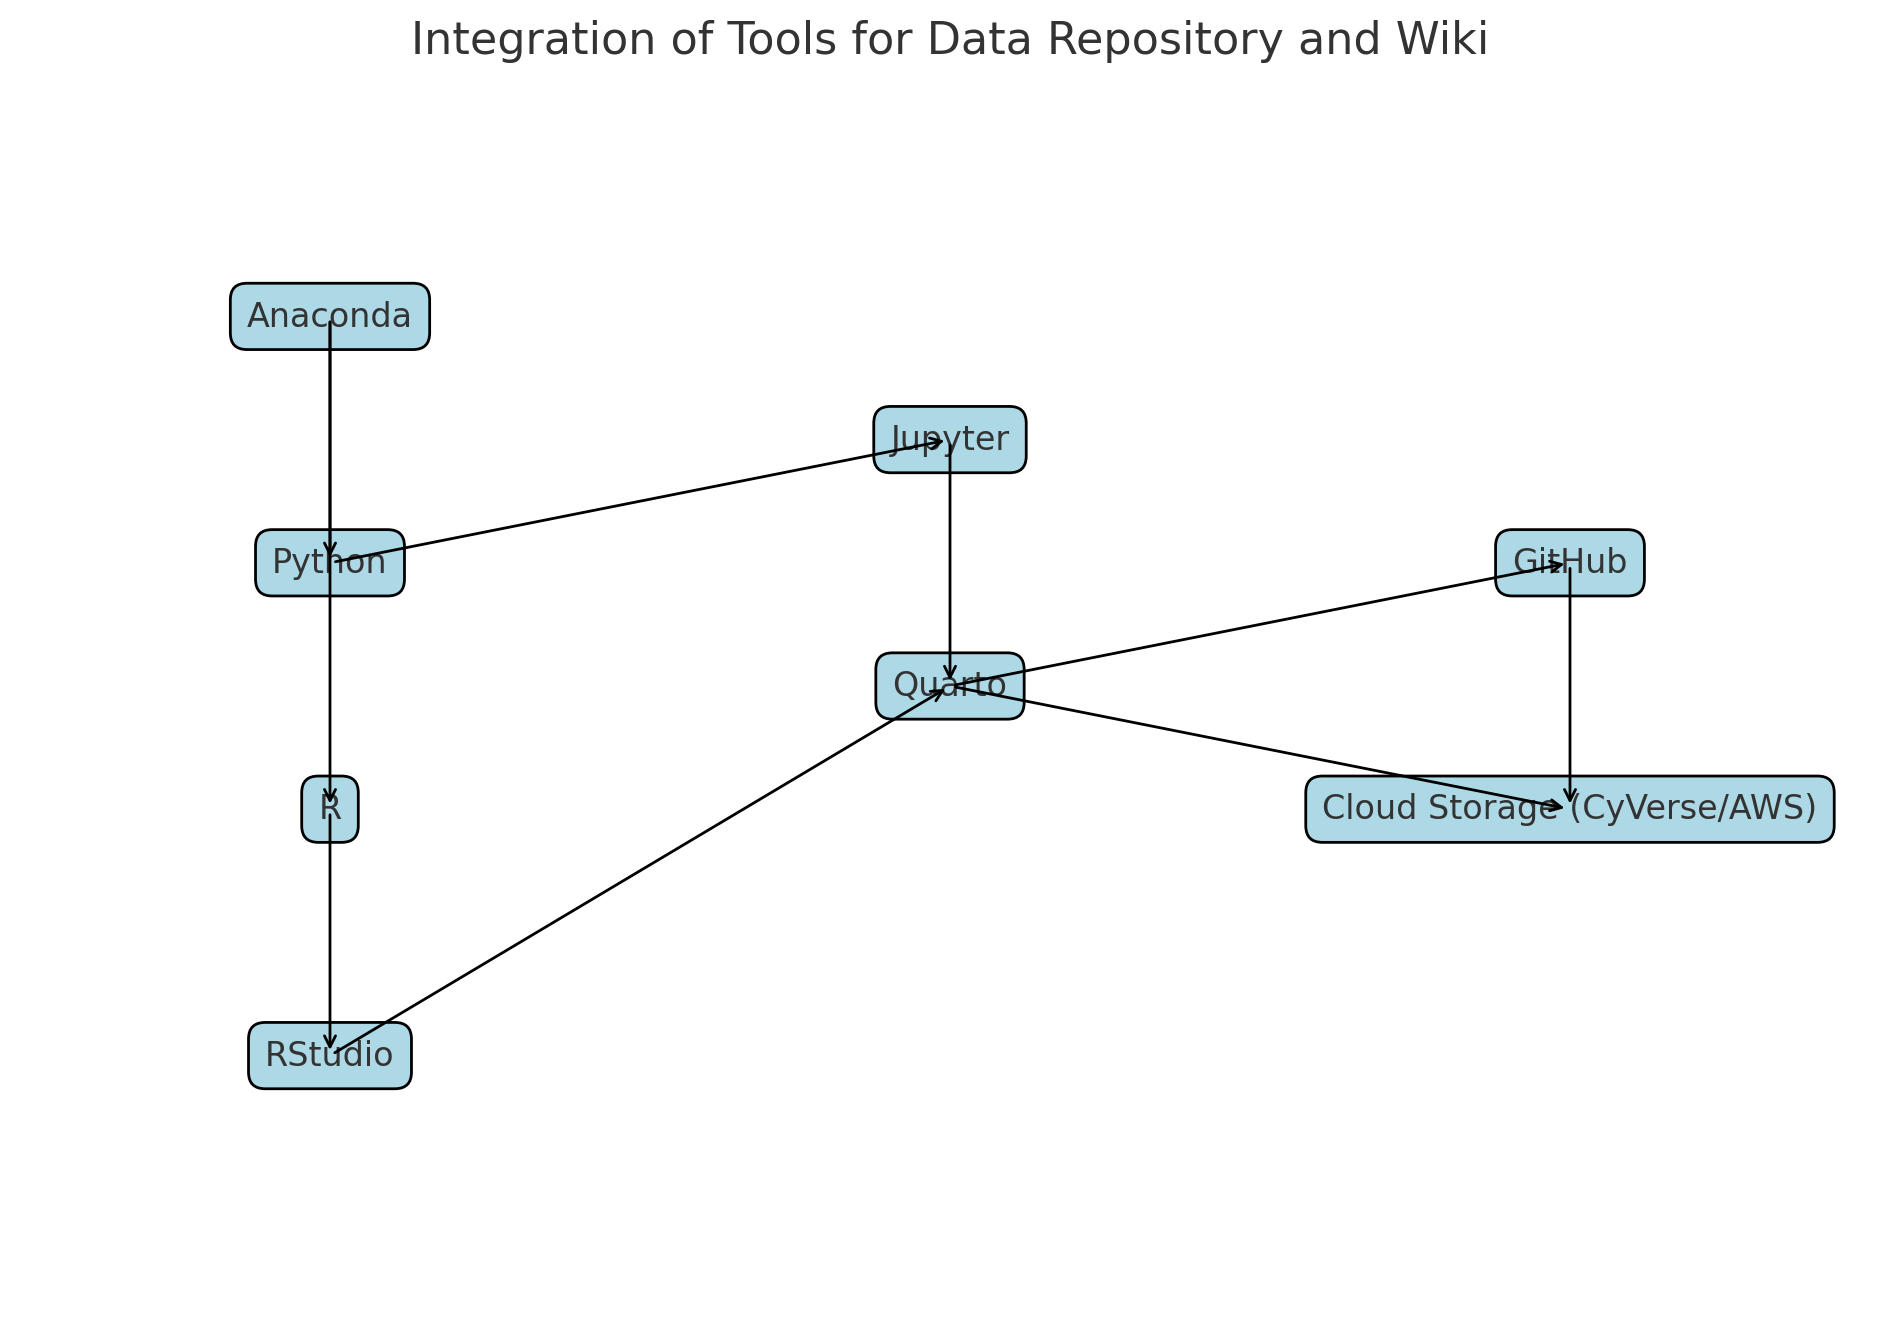
\includegraphics[width=0.9\textwidth,height=\textheight]{ecosystem_simple.png}

}

\caption{Ecosystem}

\end{figure}%

\begin{quote}
\begin{itemize}
\tightlist
\item
  \textbf{Anaconda:} Use Anaconda to create and manage your Python and R
  environments, ensuring all necessary packages are installed.
\item
  \textbf{Jupyter:} Use Jupyter Notebooks for data analysis and creating
  interactive reports. These notebooks can be converted to Quarto
  documents.
\item
  \textbf{Python:} Utilize Python's extensive libraries and tools for
  data analysis, machine learning, and visualization within Jupyter
  notebooks or standalone scripts
\item
  \textbf{R and RStudio:} Use RStudio for R-based data analysis and
  creating R Markdown documents. These can also be integrated into
  Quarto.
\item
  \textbf{Quarto:} Use Quarto to compile Jupyter Notebooks and R
  Markdown documents into a cohesive set of documentation and reports.
  Quarto can generate static websites, PDFs, and more.
\item
  \textbf{GitHub:} Host your data repository on GitHub. Use GitHub for
  version control and collaboration. Host your Quarto-generated
  documentation and wiki on GitHub Pages for easy access and sharing.
\item
  \textbf{CyVerse/AWS (Cloud Storage):} Store large files that cannot be
  accommodated on GitHub. Use CyVerse or AWS S3 to host these files and
  generate URLs for access. Include these URLs in your Quarto
  documentation, Jupyter Notebooks, and R Markdown files to provide
  seamless access to the data.
\end{itemize}
\end{quote}

\section{Getting Started}\label{getting-started}

In the next notebook I will describe how to setup this ecosystem on your
computer. Specifically using Python, Anaconda, Jupyternotebooks, Github
and Quarto

\begin{tcolorbox}[enhanced jigsaw, arc=.35mm, bottomtitle=1mm, coltitle=black, opacitybacktitle=0.6, toprule=.15mm, bottomrule=.15mm, titlerule=0mm, leftrule=.75mm, rightrule=.15mm, title=\textcolor{quarto-callout-note-color}{\faInfo}\hspace{0.5em}{Note}, opacityback=0, colframe=quarto-callout-note-color-frame, breakable, toptitle=1mm, colback=white, colbacktitle=quarto-callout-note-color!10!white, left=2mm]

Perhaps someone else can demonstrate an R-studio workflow and Cyverse
integration

\end{tcolorbox}

\href{}{link to next page}


\printbibliography


\end{document}
